\pdfminorversion=4
\documentclass[aspectratio=169]{beamer}

\mode<presentation>
{
  \usetheme{default}
  \usecolortheme{default}
  \usefonttheme{default}
  \setbeamertemplate{navigation symbols}{}
  \setbeamertemplate{caption}[numbered]
  \setbeamertemplate{footline}[frame number]  % or "page number"
  \setbeamercolor{frametitle}{fg=white}
  \setbeamercolor{footline}{fg=black}
} 

\usepackage[english]{babel}
\usepackage[utf8x]{inputenc}
\usepackage{tikz}
\usepackage{courier}
\usepackage{array}
\usepackage{bold-extra}
\usepackage{minted}
\usepackage[thicklines]{cancel}
\usepackage{fancyvrb}

\xdefinecolor{dianablue}{rgb}{0.18,0.24,0.31}
\xdefinecolor{darkblue}{rgb}{0.1,0.1,0.7}
\xdefinecolor{darkgreen}{rgb}{0,0.5,0}
\xdefinecolor{darkgrey}{rgb}{0.35,0.35,0.35}
\xdefinecolor{darkorange}{rgb}{0.8,0.5,0}
\xdefinecolor{darkred}{rgb}{0.7,0,0}
\definecolor{darkgreen}{rgb}{0,0.6,0}
\definecolor{mauve}{rgb}{0.58,0,0.82}

\title[2018-10-01-dianahep-histbook]{Histogram interoperability}
\author{Jim Pivarski}
\institute{Princeton University -- DIANA-HEP}
\date{October 1, 2018}

\usetikzlibrary{shapes.callouts}

\begin{document}

\logo{\pgfputat{\pgfxy(0.11, 7.4)}{\pgfbox[right,base]{\tikz{\filldraw[fill=dianablue, draw=none] (0 cm, 0 cm) rectangle (50 cm, 1 cm);}\mbox{\hspace{-8 cm}
\includegraphics[height=1 cm]{princeton-logo-long.png}
\includegraphics[height=1 cm]{diana-hep-logo-long.png}}}}}

\begin{frame}
  \titlepage
\end{frame}

\logo{\pgfputat{\pgfxy(0.11, 7.4)}{\pgfbox[right,base]{\tikz{\filldraw[fill=dianablue, draw=none] (0 cm, 0 cm) rectangle (50 cm, 1 cm);}\mbox{\hspace{-8 cm}
\includegraphics[height=1 cm]{princeton-logo.png}
\includegraphics[height=1 cm]{diana-hep-logo.png}}}}}

% Uncomment these lines for an automatically generated outline.
%\begin{frame}{Outline}
%  \tableofcontents
%\end{frame}

% START START START START START START START START START START START START START

\begin{frame}{Histogramming in Python}
\scriptsize
\vspace{0.25 cm}
\begin{columns}
\column{1.1\linewidth}
\renewcommand{\arraystretch}{1.2}
\begin{tabular}{c l c p{2.7 cm} p{1.5 cm} p{4.75 cm}}
pip? & name & last release & interface style & depends on & integrates with \\\hline
& \href{https://root.cern.ch/pyroot}{\textcolor{blue}{PyROOT}} & 2018 & HEP & ROOT & numpy \\
& \href{https://yoda.hepforge.org/pydoc}{\textcolor{blue}{YODA}} & 2018 & HEP & {\it compiled} & matplotlib, yaml \\
$\surd$ & \href{https://pypi.python.org/pypi/physt}{\textcolor{blue}{physt}} & 2018 & HEP + data science & numpy & pandas, xarray, dask, protobuf, matplotlib, vega (plotting), folium (maps) \\
$\surd$ & \href{https://pypi.org/project/fast-histogram}{\textcolor{blue}{fast-histogram}} & 2018 & simple (astronomy) & numpy & \\
$\surd$ & \href{https://pypi.org/project/qhist/}{\textcolor{blue}{qhist}} & 2018 & HEP & ROOT & \\
$\surd$ & \href{https://pypi.org/project/rootpy}{\textcolor{blue}{rootpy}} & 2017 & HEP & ROOT & pytables, matplotlib, stats \\
$\surd$ & \href{https://vaex.io}{\textcolor{blue}{Vaex}} (vaex.io) & 2017 & all-in-one GUI for big data, fast heatmaps & {\it many!} & Jupyter, matplotlib, HDF5, pandas, C++ \\
$\surd$ & \href{https://pypi.python.org/pypi/hdrhistogram}{\textcolor{blue}{hdrhistogram}} & 2017 & ``high dynamic range'' & {\it compiled} & Java, C++ \\
$\surd$ & \href{https://pypi.python.org/pypi/multihist}{\textcolor{blue}{multihist}} & 2017 & numpy wrapper & numpy & matplotlib \\
$\surd$ & \href{https://github.com/ibab/matplotlib-hep}{\textcolor{blue}{matplotlib-hep}} & 2016 & HEP & matplotlib & numpy, scipy \\
$\surd$ & \href{https://pypi.python.org/pypi/pyhistogram}{\textcolor{blue}{pyhistogram}} & 2014 & HEP & numpy & matplotlib, datetime \\
$\surd$ & \href{https://pypi.python.org/pypi/histogram}{\textcolor{blue}{histogram}} & 2011 & HEP & numpy & matplotlib, HDF5 \\
$\surd$ & \href{https://pypi.python.org/pypi/SimpleHist}{\textcolor{blue}{SimpleHist}} & 2011 & HEP & numpy, matplotlib & ROOT \\
$\surd$ & \href{https://pypi.org/project/paida}{\textcolor{blue}{paida}} & 2007 & HEP & & AIDA! \\
& \href{https://github.com/theodoregoetz/histogram}{\textcolor{blue}{theodoregoetz}} & never & HEP & scipy, \mbox{uncertainties} & numpy, matplotlib \\
% $\surd$ & \href{https://pypi.python.org/pypi/histogramy}{\textcolor{blue}{histogramy}} & 2013 & Numpy, Matplotlib, Scikit-Learn & & \\
% $\surd$ & \href{https://pypi.python.org/pypi/pypeaks}{\textcolor{blue}{pypeaks}} & 2014 & & & \\
% $\surd$ & \href{https://pypi.python.org/pypi/hierogram}{\textcolor{blue}{hierogram}} & 2014 & & & \\
% $\surd$ & \href{https://pypi.python.org/pypi/histo}{\textcolor{blue}{histo}} & & & & \\
% $\surd$ & \href{https://pypi.python.org/pypi/python-metrics}{\textcolor{blue}{python-metrics}} & & & & \\
% $\surd$ & \href{https://pypi.python.org/pypi/statscounter}{\textcolor{blue}{statscounter}} & 2016 & & & \\
% $\surd$ & \href{https://pypi.python.org/pypi/datagram}{\textcolor{blue}{datagram}} & & & & \\
% & \href{http://www.ifh.de/~middell/dashi/index.html}{\textcolor{blue}{dashi}} & & & & \\
\end{tabular}
\end{columns}
\end{frame}

\begin{frame}{Over the years, I've written five}
\scriptsize
\vspace{0.25 cm}
\begin{columns}
\column{1.1\linewidth}
\renewcommand{\arraystretch}{1.2}
\begin{tabular}{c l c p{2.7 cm} p{1.5 cm} p{4.75 cm}}
pip? & name & last release & interface style & depends on & integrates with \\\hline
& \href{http://code.google.com/p/plothon}{\textcolor{blue}{Plothon}} & 2006 & HEP & ROOT & SVG \\
& \href{http://code.google.com/p/svgfig}{\textcolor{blue}{SVGFig}} & 2008 & HEP & {\it none!} & SVG \\
& \href{https://github.com/opendatagroup/cassius}{\textcolor{blue}{Cassius}} & 2013 & HEP + data science & numpy & SVG, Augustus (Open Data Group) \\
$\surd$ & \href{https://github.com/histogrammar}{\textcolor{blue}{Histogrammar}} & 2016 & combinational library & numpy & Spark, Julia, CUDA, \mbox{ROOT (Cling),} matplotlib, Bokeh, Vega \\
$\surd$ & \href{https://github.com/scikit-hep/histbook}{\textcolor{blue}{histbook}} & 2018 & HEP & numpy & Spark, Pandas, Vega \\
\end{tabular}
\end{columns}

\large
\begin{uncoverenv}<2->
\vspace{1 cm}
\underline{\it Implementing} data analysis tools isn't the problem, it's designing the \underline{\it right} tool, one that solves the Cuisinart Problem:

\begin{center}
\begin{minipage}{0.8\linewidth}
It slices and dices, but is it worth the setup and cleanup?
\end{minipage}
\end{center}

Experimentation in this area is valuable.
\end{uncoverenv}
\end{frame}

\begin{frame}{All these libraries are overwhelming!}
\large
\vspace{0.5 cm}
\begin{center}
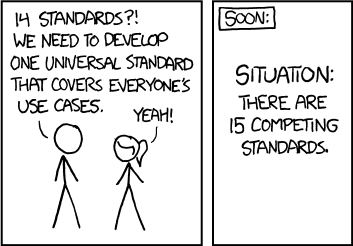
\includegraphics[width=0.4\linewidth]{standards.png}
\end{center}

\vspace{0.5 cm}
However, the real problem isn't data analysts using different tools; the problem is communicating results between data analysts.
\end{frame}

\begin{frame}{There is a standard: ROOT files}
\large
\vspace{0.5 cm}
Even if the point is to work in a non-ROOT way or to avoid ROOT dependencies, we can still share results in the ROOT file format.

\vspace{1 cm}
\textcolor{darkblue}{Look at industry:}
\begin{itemize}
\item dozens of big data SQL engines all run on Parquet files;
\item dozens of machine learning tools all run on Numpy/HDF5.
\end{itemize}

\vspace{0.25 cm}
The most conservative part of a software ecosystem is its persistence format.

\vspace{1 cm}
ROOT files are incredibly well established in HEP. It would take a strong technical argument/corner case to use something else.
\end{frame}


\end{document}
